\chapter{Positions in 2D}
\label{chapter:positions}

Positions in 2D have an x- and a y- co\"ordinate, just as a point in a graph. In Esenthel the zero point is the middle ofthe screen. Positive values on the X-axis are to the right, negative values to the left. Positive values on the Y-axis are in the upper half of the screen, negative values on the lower half.

\begin{figure}[h]
\centering
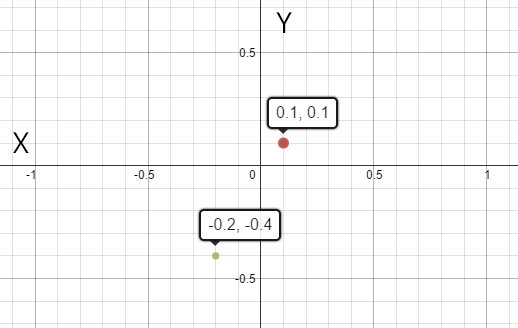
\includegraphics[width=0.7\linewidth]{../images/2Dpositions}
\caption[]{2D co\"ordinates.}
\label{fig:pos2D}
\end{figure}

In Esenthel, the class \eeClass{Vec2} is used to represent a 2D co\"ordinate. There are several ways to set the x and y values:

\begin{code}
Vec2 pos;
pos.x =  0.1; // set the x value to  0.1
pos.y = -0.3; // set the y value to -0.3
pos   =  0.5; // both x and y are set to 0.5
pos.set(0.1, -0.3); // use the function set(float x, float y) to assign both x and y
\end{code}

\section{Show a position on the screen}

Although the class \eeClass{Vec2} is mainly used to calculate positions, it is also possible to show it on the screen. This can be done with the function \eeFunc{draw(Color)}. The argument should contain the color in which the co\"ordinate must be drawn.

\begin{code}
Vec2 p1(0.2, 0.4); // Create a point p1, assigning x and y with the constructor.
Vec2 p2;           // Create a point p2.

void InitPre()
{
   EE_INIT();
}

bool Init()
{
   p2.set(-0.2, -0.5); // assign values to p2 with the set function
   return true;
}

void Shut() {}

bool Update()
{
   if(Kb.bp(KB_ESC)) return false;
   
   return true;
}

void Draw()
{
   D.clear(BLACK); // Clear the screen
   p1.draw(RED  ); // draw p1 in red  
   p2.draw(BLUE ); // draw p2 in blue
   Vec2(0 ,0).draw(GREEN); // create a temporary object and draw it in green
}

\end{code}

\section{Math}
You can do math with \eeClass{Vec2}, just as you do with plain numbers. It is possible to assign x and y values directly, but you can also do math with the class itself. In this case the operator will be applied to x as well as y:

\begin{code}
Vec2 p1(0.1,  0.3);
Vec2 p2(0.3, -0.1);
Vec2 p3 = p1 + p2;  // x: 0.4 , y: 0.2
p3 -= 0.1;          // x: 0.3 , y: 0.1
p3 *= 2;            // x: 0.6 , y: 0.2
p3 = p1 / 2.f;      // x: 0.05, y: 0.15 
\end{code}

\section{Points to remember}
The position \eeClass{Vec2(0,0)} always stands for the middle of the screen. But the borders are not always clear. Not every computer screen has the same size, but you probably want to know the border values are. For example, you want to draw something in the right corner of the screen. For this reason, Esenthel provides a few functions in the object \texttt{D} (display). You can request the width of the screen with \eeFunc{D.w()} and the height of the screen with the function \eeFunc{D.h()}. This makes it very easy to calculate the next points:

\begin{code}
Vec2 middle(0,0);
Vec2 left(-D.w(), 0);
Vec2 right(D.w(), 0);
Vec2 rightUpperCorner(D.w(), D.h());
Vec2 leftUpperCorner(-D.w(), D.h());
\end{code}

If you'd like to draw a point at a distance of 0.1 from the left upper corner, you could do that like this:

\begin{code}
Vec2(-D.w() + 0.1, D.h() - 0.1).draw(PINK);
\end{code}

\section{Summary}
\begin{itemize}
\item Points in 2D have an x- and y-co\"ordinate. In Esenthel you will use the class \eeClass{Vec2} to store a point.
\item The class \eeClass{Vec2} has a function \eeFunc{draw(Color)} to draw a point on the screen.
\item You can do math with \eeClass{Vec2}, just as with an ordinary number.
\item \eeClass{Vec2(0,0)} will always be the middle of the screen.
\item The borders of the screen can be calculated with \eeClass{D.w()} and \eeClass{D.h()}.
\end{itemize}

\section{Exercise}
Create an application which draws these points:
\begin{enumerate}
	\item A white point in the middle of the screen.
	\item A red point on 0.1 units away from the left border of the screen.
	\item A blue point on 0.2 units from the upper right corner.
	\item A yellow dot on 0.35 units from the lower border of the screen, on 2/3 of the total screen width.
\end{enumerate}
